%% bare_conf.tex
%% V1.3
%% 2007/01/11
%% by Michael Shell
%% See:
%% http://www.michaelshell.org/
%% for current contact information.
%%
%% This is a skeleton file demonstrating the use of IEEEtran.cls
%% (requires IEEEtran.cls version 1.7 or later) with an IEEE conference paper.
%%
%% Support sites:
%% http://www.michaelshell.org/tex/ieeetran/
%% http://www.ctan.org/tex-archive/macros/latex/contrib/IEEEtran/
%% and
%% http://www.ieee.org/

%%*************************************************************************
%% Legal Notice:
%% This code is offered as-is without any warranty either expressed or
%% implied; without even the implied warranty of MERCHANTABILITY or
%% FITNESS FOR A PARTICULAR PURPOSE! 
%% User assumes all risk.
%% In no event shall IEEE or any contributor to this code be liable for
%% any damages or losses, including, but not limited to, incidental,
%% consequential, or any other damages, resulting from the use or misuse
%% of any information contained here.
%%
%% All comments are the opinions of their respective authors and are not
%% necessarily endorsed by the IEEE.
%%
%% This work is distributed under the LaTeX Project Public License (LPPL)
%% ( http://www.latex-project.org/ ) version 1.3, and may be freely used,
%% distributed and modified. A copy of the LPPL, version 1.3, is included
%% in the base LaTeX documentation of all distributions of LaTeX released
%% 2003/12/01 or later.
%% Retain all contribution notices and credits.
%% ** Modified files should be clearly indicated as such, including  **
%% ** renaming them and changing author support contact information. **
%%
%% File list of work: IEEEtran.cls, IEEEtran_HOWTO.pdf, bare_adv.tex,
%%                    bare_conf.tex, bare_jrnl.tex, bare_jrnl_compsoc.tex
%%*************************************************************************

% *** Authors should verify (and, if needed, correct) their LaTeX system  ***
% *** with the testflow diagnostic prior to trusting their LaTeX platform ***
% *** with production work. IEEE's font choices can trigger bugs that do  ***
% *** not appear when using other class files.                            ***
% The testflow support page is at:
% http://www.michaelshell.org/tex/testflow/



% Note that the a4paper option is mainly intended so that authors in
% countries using A4 can easily print to A4 and see how their papers will
% look in print - the typesetting of the document will not typically be
% affected with changes in paper size (but the bottom and side margins will).
% Use the testflow package mentioned above to verify correct handling of
% both paper sizes by the user's LaTeX system.
%
% Also note that the "draftcls" or "draftclsnofoot", not "draft", option
% should be used if it is desired that the figures are to be displayed in
% draft mode.
%

% \documentclass{article}

\documentclass[conference]{IEEEtran}
\usepackage{blindtext, graphicx}
\usepackage{hyperref}
\usepackage{amsfonts}
% Add the compsoc option for Computer Society conferences.
%
% If IEEEtran.cls has not been installed into the LaTeX system files,
% manually specify the path to it like:
% \documentclass[conference]{../sty/IEEEtran}

\usepackage{amsmath,amsfonts,amssymb,amsthm,epsfig,epstopdf}

% \theoremstyle{remark}
\newtheorem{definition}{Definition}
\newtheorem{remark}[definition]{Remark}


\usepackage{algorithm}
\usepackage{algorithmic}


% Some very useful LaTeX packages include:
% (uncomment the ones you want to load)


% *** MISC UTILITY PACKAGES ***
%
%\usepackage{ifpdf}
% Heiko Oberdiek's ifpdf.sty is very useful if you need conditional
% compilation based on whether the output is pdf or dvi.
% usage:
% \ifpdf
%   % pdf code
% \else
%   % dvi code
% \fi
% The latest version of ifpdf.sty can be obtained from:
% http://www.ctan.org/tex-archive/macros/latex/contrib/oberdiek/
% Also, note that IEEEtran.cls V1.7 and later provides a builtin
% \ifCLASSINFOpdf conditional that works the same way.
% When switching from latex to pdflatex and vice-versa, the compiler may
% have to be run twice to clear warning/error messages.






% *** CITATION PACKAGES ***
%
%\usepackage{cite}
% cite.sty was written by Donald Arseneau
% V1.6 and later of IEEEtran pre-defines the format of the cite.sty package
% \cite{} output to follow that of IEEE. Loading the cite package will
% result in citation numbers being automatically sorted and properly
% "compressed/ranged". e.g., [1], [9], [2], [7], [5], [6] without using
% cite.sty will become [1], [2], [5]--[7], [9] using cite.sty. cite.sty's
% \cite will automatically add leading space, if needed. Use cite.sty's
% noadjust option (cite.sty V3.8 and later) if you want to turn this off.
% cite.sty is already installed on most LaTeX systems. Be sure and use
% version 4.0 (2003-05-27) and later if using hyperref.sty. cite.sty does
% not currently provide for hyperlinked citations.
% The latest version can be obtained at:
% http://www.ctan.org/tex-archive/macros/latex/contrib/cite/
% The documentation is contained in the cite.sty file itself.






% *** GRAPHICS RELATED PACKAGES ***
%
\ifCLASSINFOpdf
  % \usepackage[pdftex]{graphicx}
  % declare the path(s) where your graphic files are
  % \graphicspath{{../pdf/}{../jpeg/}}
  % and their extensions so you won't have to specify these with
  % every instance of \includegraphics
  % \DeclareGraphicsExtensions{.pdf,.jpeg,.png}
\else
  % or other class option (dvipsone, dvipdf, if not using dvips). graphicx
  % will default to the driver specified in the system graphics.cfg if no
  % driver is specified.
  % \usepackage[dvips]{graphicx}
  % declare the path(s) where your graphic files are
  % \graphicspath{{../eps/}}
  % and their extensions so you won't have to specify these with
  % every instance of \includegraphics
  % \DeclareGraphicsExtensions{.eps}
\fi
% graphicx was written by David Carlisle and Sebastian Rahtz. It is
% required if you want graphics, photos, etc. graphicx.sty is already
% installed on most LaTeX systems. The latest version and documentation can
% be obtained at: 
% http://www.ctan.org/tex-archive/macros/latex/required/graphics/
% Another good source of documentation is "Using Imported Graphics in
% LaTeX2e" by Keith Reckdahl which can be found as epslatex.ps or
% epslatex.pdf at: http://www.ctan.org/tex-archive/info/
%
% latex, and pdflatex in dvi mode, support graphics in encapsulated
% postscript (.eps) format. pdflatex in pdf mode supports graphics
% in .pdf, .jpeg, .png and .mps (metapost) formats. Users should ensure
% that all non-photo figures use a vector format (.eps, .pdf, .mps) and
% not a bitmapped formats (.jpeg, .png). IEEE frowns on bitmapped formats
% which can result in "jaggedy"/blurry rendering of lines and letters as
% well as large increases in file sizes.
%
% You can find documentation about the pdfTeX application at:
% http://www.tug.org/applications/pdftex





% *** MATH PACKAGES ***
%
%\usepackage[cmex10]{amsmath}
% A popular package from the American Mathematical Society that provides
% many useful and powerful commands for dealing with mathematics. If using
% it, be sure to load this package with the cmex10 option to ensure that
% only type 1 fonts will utilized at all point sizes. Without this option,
% it is possible that some math symbols, particularly those within
% footnotes, will be rendered in bitmap form which will result in a
% document that can not be IEEE Xplore compliant!
%
% Also, note that the amsmath package sets \interdisplaylinepenalty to 10000
% thus preventing page breaks from occurring within multiline equations. Use:
%\interdisplaylinepenalty=2500
% after loading amsmath to restore such page breaks as IEEEtran.cls normally
% does. amsmath.sty is already installed on most LaTeX systems. The latest
% version and documentation can be obtained at:
% http://www.ctan.org/tex-archive/macros/latex/required/amslatex/math/





% *** SPECIALIZED LIST PACKAGES ***
%
%\usepackage{algorithmic}
% algorithmic.sty was written by Peter Williams and Rogerio Brito.
% This package provides an algorithmic environment fo describing algorithms.
% You can use the algorithmic environment in-text or within a figure
% environment to provide for a floating algorithm. Do NOT use the algorithm
% floating environment provided by algorithm.sty (by the same authors) or
% algorithm2e.sty (by Christophe Fiorio) as IEEE does not use dedicated
% algorithm float types and packages that provide these will not provide
% correct IEEE style captions. The latest version and documentation of
% algorithmic.sty can be obtained at:
% http://www.ctan.org/tex-archive/macros/latex/contrib/algorithms/
% There is also a support site at:
% http://algorithms.berlios.de/index.html
% Also of interest may be the (relatively newer and more customizable)
% algorithmicx.sty package by Szasz Janos:
% http://www.ctan.org/tex-archive/macros/latex/contrib/algorithmicx/




% *** ALIGNMENT PACKAGES ***
%
%\usepackage{array}
% Frank Mittelbach's and David Carlisle's array.sty patches and improves
% the standard LaTeX2e array and tabular environments to provide better
% appearance and additional user controls. As the default LaTeX2e table
% generation code is lacking to the point of almost being broken with
% respect to the quality of the end results, all users are strongly
% advised to use an enhanced (at the very least that provided by array.sty)
% set of table tools. array.sty is already installed on most systems. The
% latest version and documentation can be obtained at:
% http://www.ctan.org/tex-archive/macros/latex/required/tools/


%\usepackage{mdwmath}
%\usepackage{mdwtab}
% Also highly recommended is Mark Wooding's extremely powerful MDW tools,
% especially mdwmath.sty and mdwtab.sty which are used to format equations
% and tables, respectively. The MDWtools set is already installed on most
% LaTeX systems. The lastest version and documentation is available at:
% http://www.ctan.org/tex-archive/macros/latex/contrib/mdwtools/


% IEEEtran contains the IEEEeqnarray family of commands that can be used to
% generate multiline equations as well as matrices, tables, etc., of high
% quality.


%\usepackage{eqparbox}
% Also of notable interest is Scott Pakin's eqparbox package for creating
% (automatically sized) equal width boxes - aka "natural width parboxes".
% Available at:
% http://www.ctan.org/tex-archive/macros/latex/contrib/eqparbox/





% *** SUBFIGURE PACKAGES ***
%\usepackage[tight,footnotesize]{subfigure}
% subfigure.sty was written by Steven Douglas Cochran. This package makes it
% easy to put subfigures in your figures. e.g., "Figure 1a and 1b". For IEEE
% work, it is a good idea to load it with the tight package option to reduce
% the amount of white space around the subfigures. subfigure.sty is already
% installed on most LaTeX systems. The latest version and documentation can
% be obtained at:
% http://www.ctan.org/tex-archive/obsolete/macros/latex/contrib/subfigure/
% subfigure.sty has been superceeded by subfig.sty.



%\usepackage[caption=false]{caption}
%\usepackage[font=footnotesize]{subfig}
% subfig.sty, also written by Steven Douglas Cochran, is the modern
% replacement for subfigure.sty. However, subfig.sty requires and
% automatically loads Axel Sommerfeldt's caption.sty which will override
% IEEEtran.cls handling of captions and this will result in nonIEEE style
% figure/table captions. To prevent this problem, be sure and preload
% caption.sty with its "caption=false" package option. This is will preserve
% IEEEtran.cls handing of captions. Version 1.3 (2005/06/28) and later 
% (recommended due to many improvements over 1.2) of subfig.sty supports
% the caption=false option directly:
%\usepackage[caption=false,font=footnotesize]{subfig}
%
% The latest version and documentation can be obtained at:
% http://www.ctan.org/tex-archive/macros/latex/contrib/subfig/
% The latest version and documentation of caption.sty can be obtained at:
% http://www.ctan.org/tex-archive/macros/latex/contrib/caption/




% *** FLOAT PACKAGES ***
%
%\usepackage{fixltx2e}
% fixltx2e, the successor to the earlier fix2col.sty, was written by
% Frank Mittelbach and David Carlisle. This package corrects a few problems
% in the LaTeX2e kernel, the most notable of which is that in current
% LaTeX2e releases, the ordering of single and double column floats is not
% guaranteed to be preserved. Thus, an unpatched LaTeX2e can allow a
% single column figure to be placed prior to an earlier double column
% figure. The latest version and documentation can be found at:
% http://www.ctan.org/tex-archive/macros/latex/base/



%\usepackage{stfloats}
% stfloats.sty was written by Sigitas Tolusis. This package gives LaTeX2e
% the ability to do double column floats at the bottom of the page as well
% as the top. (e.g., "\begin{figure*}[!b]" is not normally possible in
% LaTeX2e). It also provides a command:
%\fnbelowfloat
% to enable the placement of footnotes below bottom floats (the standard
% LaTeX2e kernel puts them above bottom floats). This is an invasive package
% which rewrites many portions of the LaTeX2e float routines. It may not work
% with other packages that modify the LaTeX2e float routines. The latest
% version and documentation can be obtained at:
% http://www.ctan.org/tex-archive/macros/latex/contrib/sttools/
% Documentation is contained in the stfloats.sty comments as well as in the
% presfull.pdf file. Do not use the stfloats baselinefloat ability as IEEE
% does not allow \baselineskip to stretch. Authors submitting work to the
% IEEE should note that IEEE rarely uses double column equations and
% that authors should try to avoid such use. Do not be tempted to use the
% cuted.sty or midfloat.sty packages (also by Sigitas Tolusis) as IEEE does
% not format its papers in such ways.





% *** PDF, URL AND HYPERLINK PACKAGES ***
%
%\usepackage{url}
% url.sty was written by Donald Arseneau. It provides better support for
% handling and breaking URLs. url.sty is already installed on most LaTeX
% systems. The latest version can be obtained at:
% http://www.ctan.org/tex-archive/macros/latex/contrib/misc/
% Read the url.sty source comments for usage information. Basically,
% \url{my_url_here}.





% *** Do not adjust lengths that control margins, column widths, etc. ***
% *** Do not use packages that alter fonts (such as pslatex).         ***
% There should be no need to do such things with IEEEtran.cls V1.6 and later.
% (Unless specifically asked to do so by the journal or conference you plan
% to submit to, of course. )

\newcommand{\R}{\mathbb{R}}

% correct bad hyphenation here
\hyphenation{op-tical net-works semi-conduc-tor}


\begin{document}
%
% paper title
% can use linebreaks \\ within to get better formatting as desired
\title{Course Project: Dynamic Programming on Tensors for Solving the Problem of Dependency Parsing in NLP}


% author names and affiliations
% use a multiple column layout for up to three different
% affiliations
\author{\IEEEauthorblockN{Sergey Divakov\IEEEauthorrefmark{1},
Anastasia Koloskova\IEEEauthorrefmark{2}, Alfredo De la Fuente \IEEEauthorrefmark{3} and
Vladislav Pimanov\IEEEauthorrefmark{4}}
\IEEEauthorblockA{Data Science Department,
Skolkovo Institute of Science and Technology\\
Moscow, Russia\\
Email: \IEEEauthorrefmark{1}Sergei.Divakov@skoltech.ru,
\IEEEauthorrefmark{2}Anastasiia.Koloskova@skoltech.ru,\\
\IEEEauthorrefmark{3}Alfredo.DeLaFuente@skoltech.ru,
\IEEEauthorrefmark{4}Vladislav.Pimanov@skoltech.ru}}

% conference papers do not typically use \thanks and this command
% is locked out in conference mode. If really needed, such as for
% the acknowledgment of grants, issue a \IEEEoverridecommandlockouts
% after \documentclass

% for over three affiliations, or if they all won't fit within the width
% of the page, use this alternative format:
% 
%\author{\IEEEauthorblockN{Michael Shell\IEEEauthorrefmark{1},
%Homer Simpson\IEEEauthorrefmark{2},
%James Kirk\IEEEauthorrefmark{3}, 
%Montgomery Scott\IEEEauthorrefmark{3} and
%Eldon Tyrell\IEEEauthorrefmark{4}}
%\IEEEauthorblockA{\IEEEauthorrefmark{1}School of Electrical and Computer Engineering\\
%Georgia Institute of Technology,
%Atlanta, Georgia 30332--0250\\ Email: see http://www.michaelshell.org/contact.html}
%\IEEEauthorblockA{\IEEEauthorrefmark{2}Twentieth Century Fox, Springfield, USA\\
%Email: homer@thesimpsons.com}
%\IEEEauthorblockA{\IEEEauthorrefmark{3}Starfleet Academy, San Francisco, California 96678-2391\\
%Telephone: (800) 555--1212, Fax: (888) 555--1212}
%\IEEEauthorblockA{\IEEEauthorrefmark{4}Tyrell Inc., 123 Replicant Street, Los Angeles, California 90210--4321}}




% use for special paper notices
%\IEEEspecialpapernotice{(Invited Paper)}


% make the title area
\maketitle

\begin{abstract}
%\boldmath
As part of the Optimization Methods - Numerical Linear Algebra courses final project, we explore the benefits of using tensor decomposition in order to reduce the asymptotically complexity of the well-known dynamic programming algorithm Inside-Outside (marginal probabilities computation) to infer PCFG grammars and improve the performance at parsing tasks. We benchmark our parsing quality with appropriate metric as well as the implementation speed using the treebank datasets available. We observe significant improvements by incorporating the proposed methodology.


\end{abstract}
% IEEEtran.cls defaults to using nonbold math in the Abstract.
% This preserves the distinction between vectors and scalars. However,
% if the journal you are submitting to favors bold math in the abstract,
% then you can use LaTeX's standard command \boldmath at the very start
% of the abstract to achieve this. Many IEEE journals frown on math
% in the abstract anyway.

% Note that keywords are not normally used for peerreview papers.
\begin{IEEEkeywords}
Tensor decomposition, dynamic programming, NLP.
\end{IEEEkeywords}



% For peer review papers, you can put extra information on the cover
% page as needed:
% \ifCLASSOPTIONpeerreview
% \begin{center} \bfseries EDICS Category: 3-BBND \end{center}
% \fi
%
% For peerreview papers, this IEEEtran command inserts a page break and
% creates the second title. It will be ignored for other modes.
\IEEEpeerreviewmaketitle



\section{Introduction}
Syntactic dependency parsing is one of the major problems in statistical natural language processing.  There exists many algorithms to solve this problem, but we will focus on Probabilistic Contex Free Grammars (PCFG) with latent states, which is one of the most successful and mathematically interesting approaches.

Latent variable models have shown promising results in different areas in computational linguistics, bioinformatics and machine learning. Many different approaches have been recently suggested to solve the syntactic parsing task (spectral learning \cite{IEEEhowto:narayan}, recursive neural networks \cite{IEEEhowto:socher}), however regardless of the learning algorithm, the inference always relies on the inside-outside algorithm, which is a dynamic programming algorithm, allowing to calculate the marginal probabilities for spans of the parse tree.

The Inside-Outside algorithm has cubic complexity in the cardinality of non-terminal symbols. 
There is, however, a way to reformulate this problem in terms of dynamic programming on a tensor, with each step corresponding to some contraction. A relatively recent paper \cite{IEEEhowto:cohen} uses this approach and applies the canonical tensor decomposition to reduce the complexity of the inference to linear in the number of non-terminals, with only a slight decrease in quality. Our goal is to try to improve on this result by testing different methods for tensor decomposition (Tucker and Tensor Train) and evaluate the quality of approximation both in terms of speed and precision.

In our project we will provide some basic notions regarding PCFGs and tensor decomposition methods; in order to implement the algorithm, perform different experiments and evaluate results.

\section{Setup}

For an integer $n \geq 1$, we let $[n] = \{1, 2, \dots, n\}$.


\subsection{Probabilistic Context-Free Grammars}
We consider a probabilistic context-free grammar (PCFG) $G$ in Chomsky normal form, which can be defined by a quintuple
\begin{equation}
    G = (\mathcal{N}, \mathcal{L}, \mathcal{R},\mathcal P, \pi),
\end{equation}
where 

\begin{enumerate}
    \item $\mathcal{N}$ is the finite set of nonterminal symbols, $|\mathcal{N}| = m$.
    \item $\mathcal{L}$ is the finite set of words (lexical tokens), $| \mathcal{L}| = n$.
    \item $\mathcal{R}$ is a set of rules: $a \to bc$ or $a \to x$, where $a, b, c \in \mathcal{N}$, $x \in \mathcal{L}$.
    \item $\mathcal{P}$ is a transition probability distribution: for each $(a \to x) \in \mathcal{R}$ and $a\to bc \in \mathcal{R}$ we have a parameter $p(a \to bc | a)$ and $p(a\to x|a)$.
    \item $\pi$ is an probability distribution for non-terminal symbols. For each $a \in \mathcal{N}$ we have $\pi_a$ which is a probability of $a$ being the root symbol of a derivation. 
    
\end{enumerate}

The parameters above satisfy the following normalization conditions:
$$ \sum_{(a\to bc) \in \mathcal{R}} p(a\to bc|a) + \sum_{(a\to x) \in \mathcal{R}}p(a\to x|a) = 1,$$
for each $a \in \mathcal{N}$, and $\sum_{a\in \mathcal{N}}\pi_a = 1$.

\subsection{Tensor}
\begin{definition}[Tensor]
A Tensor $T \in \R^{m\times m \times m}$ is a set of $m^3$ parameters $T_{i,j,k}$ for $i, j, k \in [m]$.

\end{definition}

\begin{definition}[Tensor Contraction]
Given a tensor $T \in \R^{m\times m\times m}$ and vectors $v^1, v^2 \in \R^m$ we define a tensor contraction $T_{(1,2)} \in \R^{m\times m \times m}$ which is the function
$T_{(1,2)}:\R^m\times \R^m \to \R^{1\times m}$ defined as $T(v_1,v_2)_k = \sum_{i,j}
T_{ijk}v^1_iv^2_j$. Similarly, contractions $T_{(1,3)}$ and $T_{(2,3)}$ are defined.
\end{definition}

We use tensor representation of transition probabilities in grammar $G$ and we denote by $T \in \R^{m\times m \times m}$ a tensor such that $$T_{a,b,c} = p(a\to bc|a).$$
Similarly, we denote by $Q\in \R^{m\times n}$ a matrix such that 
$$Q_{a,x} = p(a\to x| a).$$
Also, we introduce probabilities of each non-terminal to be a root, we denote it using a vector $\pi \in \R^{m\times 1}$ such that $\pi_a$ is a probability of $a$ to be a root.

\subsection{Parsing}

Parsing is the process of taking a string and a grammar and find a derivation from start category $S$ for the input string, in other words, assigning proper trees to input strings based on the rules established by the grammar. 

We must notice than often a sentence can give us an ambiguous parse, then how do we choose the best tree among all those returned? To solve this issue, we can assign probability values (weights) to the set of rules (PCFG) and rank parses by combining their weights. These probabilities can be learned from an annotated corpus (treebank) by using the inside-outside algorithm.


\begin{figure}
  \centering
  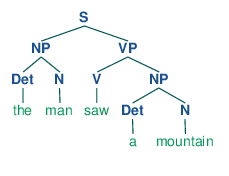
\includegraphics[ width=0.7\linewidth]{img1.png}
  \caption{Parse tree representation of  \textit{the man saw a mountain}}
  \centering
  \label{fig:boat1}
\end{figure}


\begin{definition}[Parse Tree] Let $z = x_1 \dots x_N$ be an input sentence. We denote by $\tau$ a parse tree of given sentence. The root of $\tau$ is $S$, leaves are terminal symbols $x_1\dots x_N$. If tree node $A$ has two children $B$ and $C$ then the rule $A\to BC$ is present in our grammar $G$, i.e. $A \to BC \in \mathcal{R}$ (see fig. \ref{fig:boat1}).

The set of all possible trees $\tau$ for given input string $z$ we denote as $\mathcal{T}(z)$.
\end{definition}

\section{Parsing Algorithm}

% In this section we describe dynamic programming algorithm for parsing string of tokens. 
\subsection{Minimum Bayes-Risk Decoding}

According to previous definition, parsing of string $z$ is choosing the "best" parsing tree $\tau$ from all possible parsing trees $\mathcal{T}(z)$.
In our project parsing aims to find the highest scoring tree $\tau^*$ for $z$ according to the underlying PCFG, also called "Viterbi parse":
\begin{equation}\label{eq:hs_tree}
   \tau^* = \arg\max_{\tau \in \mathcal{T}(z)} p(\tau).  
\end{equation}
Goodman suggested dynamic programming approach, called "Labelled Recall Algorithm" \cite{IEEEhowto:goodman}, which aims to find the highest scoring tree \eqref{eq:hs_tree}.

This algorithm has two phases. At the first phase it computes marginals which are defined as 
$$ \mu(a, i, j) = \sum_{\tau \in \mathcal{T}(z): (a, i, j) \in \tau} p(\tau),$$
where $(a, i, j) \in \tau$ denotes that nonterminal $a$ spans words $x_i\dots x_j$ in the parse tree $\tau$.

The second phase includes a dynamic programming algorithm which finds a tree $\tau^*$ that maximized the sum over marginals in that tree:
$$ \tau^* = \arg\max_{\tau\in \mathcal{T}(z)} \sum_{(a,i,j)\in \tau} \mu(a,i,j).$$
Goodman’s algorithm is described in Algorithm \ref{alg:label_recall}. 

\begin{algorithm}[h!]
   \caption{Labelled Recall Algorithm}
   \label{alg:label_recall}
\begin{algorithmic}
    \STATE{\bfseries Inputs:} Sentence $x_1 \dots x_N$,     PCFG$(\mathcal{N},\mathcal{L, R})$, parameters $T \in \R^{m\times m\times m}$, $Q \in \R^{m\times m}$, $\pi \in \R^{m\times1}$.
    \STATE{\bfseries Marginals:} $\forall a \in \mathcal{N}$, $\forall i, j\in [N], i \leq j$ compute the marginals $\mu(a,i,j)$ using the inside-outside algorithm.
    \STATE{\bfseries Base case:} $\forall i \in [N]$,
    $$\gamma^{i,i} = \max_{(a\to x_i)\in\mathcal{R}} \mu(a,i,i).$$
    \STATE{\bfseries Maximize Labelled Recall:} $\forall i,j \in [N], i < j,$
    $$\gamma^{i,j} = \max_{a\in \mathcal{N}}\mu(a,i,j) + \max_{i\leq k < j}(\gamma^{i,k} + \gamma^{k+1, j}).$$
\end{algorithmic}
\end{algorithm}

\subsection{Inside-Outside Algorithm}
The representation of the inside-outside algorithm
in tensor form for calculation of marginal terms $\mu(a,i,j)$.
\begin{algorithm}[h!]
\caption{Inside-Outside Algorithm}
\label{alg:inside-outside}
\begin{algorithmic}
    \STATE{\bfseries Inputs:} Sentence $x_1 \dots x_N$,
    PCFG$(\mathcal{N},\mathcal{L, R})$, parameters $T \in \R^{m\times m\times m}$, $Q \in \R^{m\times m}$, $\pi \in \R^{m\times1}$.
    
    \STATE{\bfseries Data Structures:} 
    \begin{itemize}
        \item $\alpha^{i,j} \in \R^{1\times m}$,
    $i,j \in [N],$ $i \leq j$, is a row vector representing inside terms ranging over $a \in \mathcal{N}$.
        \item $\beta^{i,j} \in \R^{m\times 1}$,
    $i,j \in [N],$ $i \leq j$, is a column vector representing outside terms ranging over $a \in \mathcal{N}$.
    \end{itemize}
    
    \STATE{\bfseries Inside Base Case:} $\forall i \in [N], \forall(a \to x_i) \in \mathcal{R}$:
    
    $[\alpha^{i,i}]_a = Q_{a,x}$
    \STATE{\bfseries Inside Recursion:} $\forall i,j \in [N]$, $i < j$:
    
    $[\alpha^{i,j}]_a = \sum_{k=i}^{j-1} T_{(2,3)}(\alpha^{i,k},\alpha^{k+1,j})$
    \STATE{\bfseries Outside Base Case:} $\forall a \in \mathcal{N}$:
    
    $[\beta^{1,N}]_a = \pi_a$
    \STATE{\bfseries Outside Recursion:} $\forall i,j \in [N]$, $i \leq j$:
    
    $\beta^{i,j} = \sum_{k=1}^{i-1} T_{(1,2)}(\beta^{k,j},\alpha^{k,i-1}$  
    
    $+ \sum_{k=j+1}^{N} T_{(1,3)}(\beta^{i,k},\alpha^{j+1,k})$
    \STATE{\bfseries Marginals:} $\forall a \in \mathcal{N}$, $ \forall i,j \in [N]$, $i \leq j$:
    
    $ \mu(a,i,j) = [\alpha^{i,j}]_a \cdot [\beta^{i,j}]_a$
\end{algorithmic}
\end{algorithm}

Time complexity of the inside-outside algorithm is $\mathcal{O}(m^3N^3)$,
since each naive tensor contraction takes time $\mathcal{O}(m^3)$.
To reduce the complexity we approximate parsing using different tensor decompostions.

\section{Tensor Decompositions}
In this section we provide an overview of three tensor decomposition methods: canonical decomposition, Tucker decomposition and Tensor Train decomposition. Using any of these decompositions we can multiply tensor-by-vectors is linear in $m$ time instead of cubic complexity for naive multiplication. 

\subsection{Canonical Decomposition}
The canonical polyadic decomposition (CPD), also known as tensor rank decomposition, is basically a generalization of SVD to tensors. In that way, we can represent a order $d$ tensor $\mathcal{A} \in \mathbb{R}^{n_1 \times n_2 \times \dots n_d } $ as a linear combination of $r$ pure rank tensors as follows,
$$ \mathcal{A} = \sum_{i=1}^r \lambda_i \textbf{a}_i^1 \otimes \textbf{a}_i^2 \otimes \dots \textbf{a}_i^d $$
% TODO: AK: write what \otimes represent here? 
where $\lambda_i \in \mathbb{R} $ and $\textbf{a}_i^j \in \mathbb{R}^{n_j}$. In practice this decomposition is computed by using different optimization methods such as Levenber - Marquardt (LM), nonlinear conjugate gradient (NCG) or Broyden-Fletcher-Goldfarb-Shanno (BFGS); or by using alternating least squares (ALS).


\begin{remark}[Complexity of Tensor Contraction]
Let $\mathcal{A} \in \R^{m\times m\times m}$ be a 3-dimensional tensor represented in the canonical decomposition form, $v_1, v_2 \in \R^m$. The complexity of computing contraction of $\mathcal{A}$ and $v_1, v_2$ is $\mathcal{O}(rm)$.
\end{remark}

\subsection{Tucker Decomposition}
Tucker decomposition decomposes a tensor into a set of matrices and one small core tensor. That is, for a tensor $\mathcal{A} \in \mathbb{R}^{ n_1 \times n_2 \times n_3} $, its Tucker decomposition is given by
$$ \text{vec} ( \mathcal{A}  ) =  \left( W \otimes V \otimes U \right) \cdot \text{vec} ( \mathcal{C} ) $$
where, $vec$ is the vectorization operator, with $U \in \mathbb{R}^{n_1\times r_1}$, $V \in \mathbb{R}^{n_2\times r_2}$, $W \in \mathbb{R}^{n_3\times r_3}$ and the core tensor $\mathcal{C}\in \mathbb{R}^{r_1 \times r_2 \times r_3}$.

\begin{remark}[Complexity of Tensor Contraction]
Let $\mathcal{A} \in \R^{m\times m\times m}$ be a 3-dimensional tensor in the Tucker decomposition form, $v_1, v_2 \in \R^m$. The complexity of computing contraction of $\mathcal{A}$ and $v_1, v_2$ is $\mathcal{O}(rm + r^3)$.
\end{remark}

\subsection{Tensor Train Decomposition}
Tensor Train (TT) decomposition is a representation of $d$-tensor $\mathcal{A} \in \mathbb{R}^{n_1 \times n_2 \times \dots n_d } $ in the following way:
\begin{equation*}
\begin{aligned}
    \mathcal{A}(i_1,\ldots,i_d) = \\\sum
    g_1(\alpha_0,i_1,\alpha_1)g_2(\alpha_1,i_2,\alpha_2)\times\ldots\times\\ g_{d-1}(\alpha_{d-2},i_{d-1},\alpha_{d-1})g_d(\alpha_{d-1},i_d,\alpha_d)
\end{aligned}
\end{equation*}
where summation is on the indices $\alpha_k$, which are repeated exactly twice.
Let $\alpha_k$ varies from $1$ to $r_k$, then $r_1,\ldots,r_{d-1}$ are ranks of TT
decomposition. 

\begin{remark}[Complexity of Tensor Contraction]
Let $\mathcal{A} \in \R^{m\times m\times m}$ be a 3-dimensional tensor in the TT form, $v_1, v_2 \in \R^m$. The complexity of computing contraction of $\mathcal{A}$ and $v_1, v_2$ is $\mathcal{O}(mr^2)$.
\end{remark}


% needed in second column of first page if using \IEEEpubid
%\IEEEpubidadjcol

% An example of a floating figure using the graphicx package.
% Note that \label must occur AFTER (or within) \caption.
% For figures, \caption should occur after the \includegraphics.
% Note that IEEEtran v1.7 and later has special internal code that
% is designed to preserve the operation of \label within \caption
% even when the captionsoff option is in effect. However, because
% of issues like this, it may be the safest practice to put all your
% \label just after \caption rather than within \caption{}.
%
% Reminder: the "draftcls" or "draftclsnofoot", not "draft", class
% option should be used if it is desired that the figures are to be
% displayed while in draft mode.
%
%\begin{figure}[!t]
%\centering
%\includegraphics[width=2.5in]{myfigure}
% where an .eps filename suffix will be assumed under latex, 
% and a .pdf suffix will be assumed for pdflatex; or what has been declared
% via \DeclareGraphicsExtensions.
%\caption{Simulation Results}
%\label{fig_sim}
%\end{figure}

% Note that IEEE typically puts floats only at the top, even when this
% results in a large percentage of a column being occupied by floats.


% An example of a double column floating figure using two subfigures.
% (The subfig.sty package must be loaded for this to work.)
% The subfigure \label commands are set within each subfloat command, the
% \label for the overall figure must come after \caption.
% \hfil must be used as a separator to get equal spacing.
% The subfigure.sty package works much the same way, except \subfigure is
% used instead of \subfloat.
%
%\begin{figure*}[!t]
%\centerline{\subfloat[Case I]\includegraphics[width=2.5in]{subfigcase1}%
%\label{fig_first_case}}
%\hfil
%\subfloat[Case II]{\includegraphics[width=2.5in]{subfigcase2}%
%\label{fig_second_case}}}
%\caption{Simulation results}
%\label{fig_sim}
%\end{figure*}
%
% Note that often IEEE papers with subfigures do not employ subfigure
% captions (using the optional argument to \subfloat), but instead will
% reference/describe all of them (a), (b), etc., within the main caption.


% An example of a floating table. Note that, for IEEE style tables, the 
% \caption command should come BEFORE the table. Table text will default to
% \footnotesize as IEEE normally uses this smaller font for tables.
% The \label must come after \caption as always.
%
%\begin{table}[!t]
%% increase table row spacing, adjust to taste
%\renewcommand{\arraystretch}{1.3}
% if using array.sty, it might be a good idea to tweak the value of
% \extrarowheight as needed to properly center the text within the cells
%\caption{An Example of a Table}
%\label{table_example}
%\centering
%% Some packages, such as MDW tools, offer better commands for making tables
%% than the plain LaTeX2e tabular which is used here.
%\begin{tabular}{|c||c|}
%\hline
%One & Two\\
%\hline
%Three & Four\\
%\hline
%\end{tabular}
%\end{table}


% Note that IEEE does not put floats in the very first column - or typically
% anywhere on the first page for that matter. Also, in-text middle ("here")
% positioning is not used. Most IEEE journals use top floats exclusively.
% Note that, LaTeX2e, unlike IEEE journals, places footnotes above bottom
% floats. This can be corrected via the \fnbelowfloat command of the
% stfloats package.

\section{Methodology}

The full implementation of the project is open source available in the following  \href{https://github.com/divserge/pcfg_parser}{GitHub repository}. All the scripts and notebooks reproducing the results can also be found there.


\section{Experiments}
\subsection{Data}

We used a section of the Penn TreeBank (PTB) \cite{IEEEhowto:marcus} obtained from Wall Street Journal (WSJ). The Natural Language Toolkit (NLTK) let us access to a $5\%$ fragment of the PTB corpus (about 1,600 sentences), which we used to familiarize with the task and train simple latent-variable parsing model using the expectation-maximization algorithm. In order to test our methodology, we considered the  \href{http://cohort.inf.ed.ac.uk/lpcfg.html}{Multilingual L-PCFG Models} dataset. We focused our analysis on the French grammar section to run our experiments.


\subsection{Evaluation}
The most common parsing evaluation metrics examine the conceptual "distance" between the candidate parse generated by the parser, and the correctly annotated solution (the \textit{gold standard}). Gold standards are sometimes annotated by hand, but more often they are inferred from existing corpora.

The current standard comparison is the ParseEval metric \cite{IEEEhowto:Black}. It defines a set of values that focus primarily on the constituency differences between the two trees. The idea of this metric is straightforward: measure the \textit{exact match}, i.e. proportion of gold standard trees that parser got right. 

ParseEval metric computes two values: \textbf{precision} and \textbf{recall}. 
To compute precision it finds proportion of constituents in \textit{parse tree} which are also present in \textit{gold tree}.
To compute recall it finds proportion of constituents in \textit{gold tree} which are also present in \textit{parse tree}.

You can see example on the fig. \ref{fig:precision-recall}
\begin{figure}[H]
      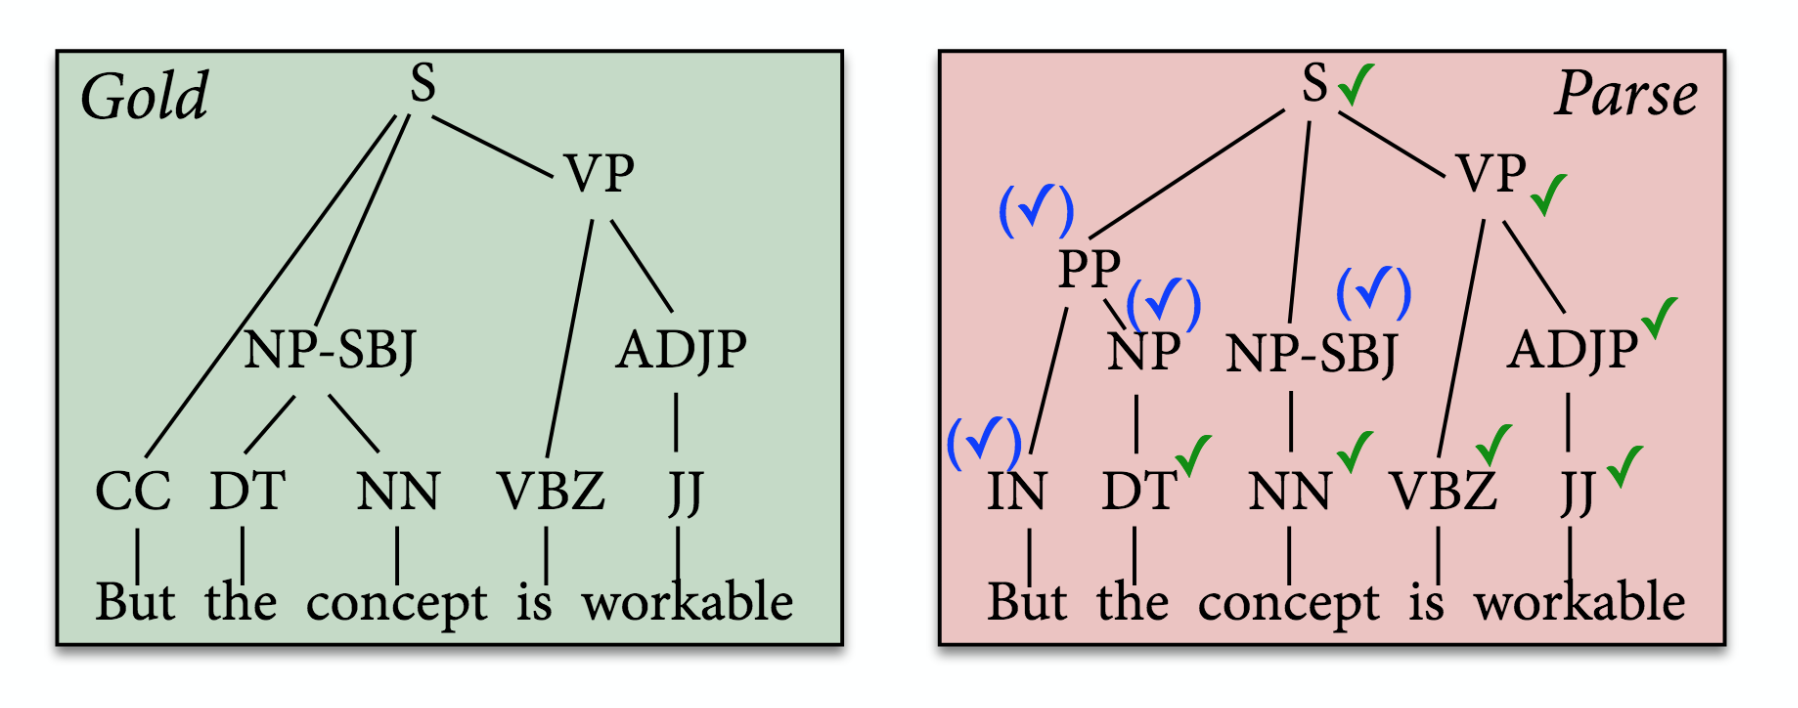
\includegraphics[ width=\linewidth, height=0.3\linewidth]{precision.png}
      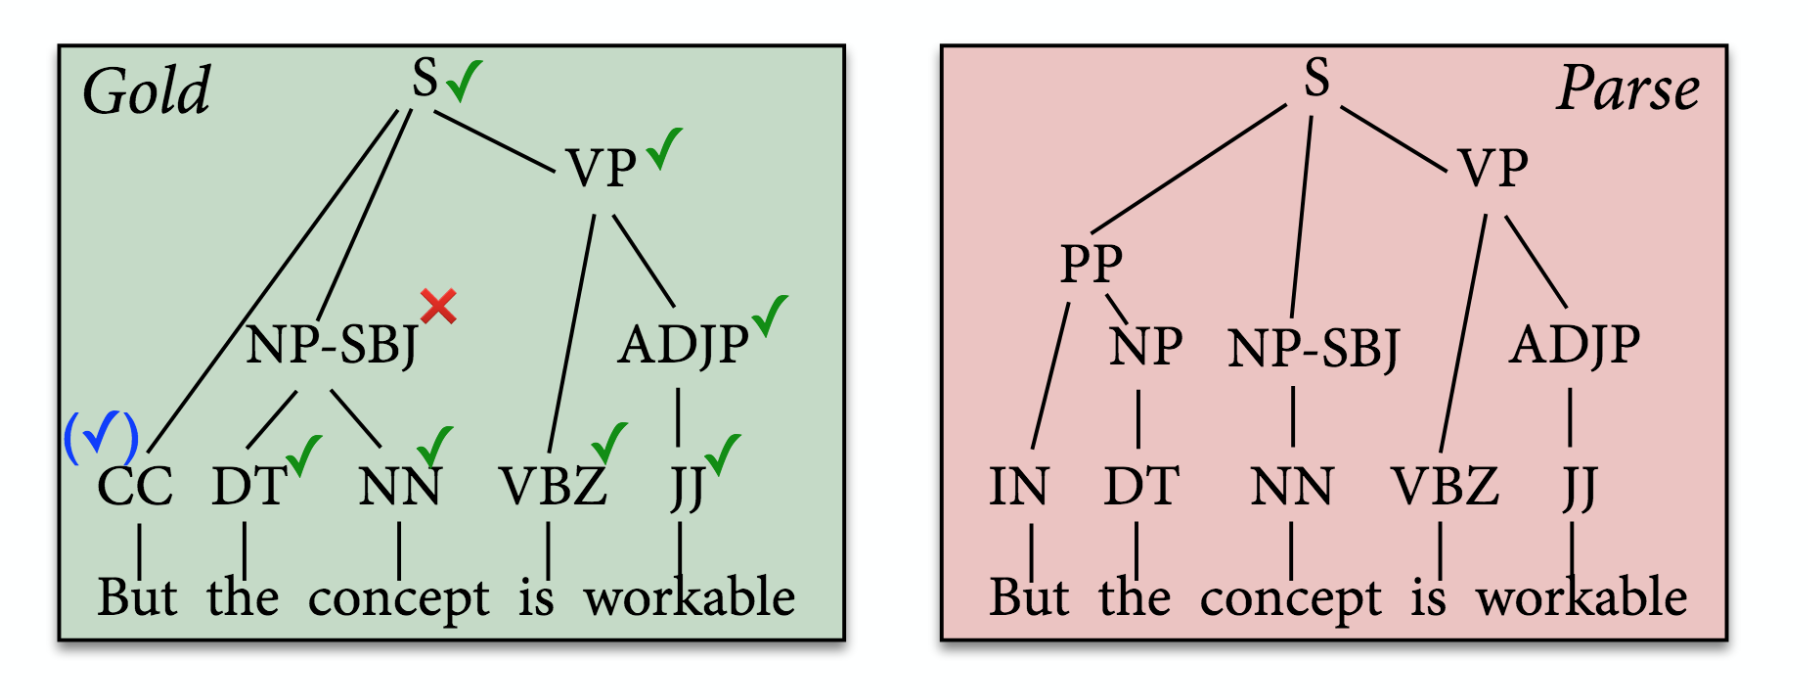
\includegraphics[ width=\linewidth, height=0.3\linewidth]{recall.png}
      \caption{Computing Precision (top) and Recall (bottom).}
      \centering\label{fig:precision-recall}
\end{figure}
After computing precision $p$ and recall $r$, we can easily compute the  $f_1$ score by 
$$f_1 = \dfrac{2\ p\ r}{p + r},$$

\subsection{Results}

We performed a sequence of tests to benchmark, with respect to time and accuracy, our proposed methodology in comparison to the base line (inside outside with no tensors). We begin by comparing both Tucker and Tensor Train decomposition algorithms in the approximating syntactic parse task. We run both approaches fixing the ranks of the tensor decomposition to be $10$, $50$ and $100$. We observe the results plotted in figures, \ref{fig:tt10} and \ref{fig:tt100}. 

\begin{figure}[H]
  \centering
  \includegraphics[width=.8\linewidth]{test_tt_10.png}
  \caption{Distribution of F1 scores for rank 10 - Tensor Train decomposition}
  \label{fig:tt10}
\end{figure}%
\begin{figure}[H]
  \centering
  \includegraphics[width=.8\linewidth]{test_tt_100.png}
  \caption{Distribution of F1 scores for rank 100 - Tensor Train decomposition}
  \label{fig:tt100}
\end{figure}

We can observe a slightly better performance of Tensor Train decomposition approach compared to Tucker, however both seem to significantly obtain a remarkable F1-score performance for parsing the sentences in our french dataset considered. We obtained for rank $100$ an average F1-score of $0.8095$ for Tucker decomposition and $0.8103$ for Tensor Train decomposition. For TT decompositions with rank over 150 the F1-score is equal to 1.0, meaning that the parsing is exact, however we still observe a significant speed improvement for such ranks.

In addition, we run several experiments to find how time complexity of our methodology relates to the size of the rank we will use to approximate our tensor. In fig. \ref{fig:tests_time} we observe a substantial improvement in time performance. The gap in performance time maintains for different rank approximations used, which proves the main hypothesis of our research, without compromising accuracy. 

\begin{figure}[H]
\centering
 \includegraphics[width=.8\linewidth]{tt-time.png}
\caption{Time benchmark - Tensor Train decomposition vs baseline method.}
\label{fig:tests_time}
\end{figure}

\section{Conclusion}

We described and implemented a tensor decomposition approach for probabilistic context-free parsing. The scheme presented leads to a speed-up in PCFG parsing with minimal loss in accuracy using ParseEval metric.


% if have a single appendix:
%\appendix[Proof of the Zonklar Equations]
% or
%\appendix  % for no appendix heading
% do not use \section anymore after \appendix, only \section*
% is possibly needed

% use appendices with more than one appendix
% then use \section to start each appendix
% you must declare a \section before using any
% \subsection or using \label (\appendices by itself
% starts a section numbered zero.)
%

% use section* for acknowledgement
\section*{Acknowledgment}


The authors would like to thank the guidance and patience of the teaching assistants assigned to contribute in our group.


\section*{Contribution}

\begin{itemize}
    \item[] \textbf{Sergey Divakov} \\
    Idea, architecture and uniting all parts of the parser code. Implementing Labelled Recall Algorithm and Inside-Outside algorithm with tensor train. Also implemented em-algorithm for training the pcfgs. Conducting numerical experiments, contribution to the presentation and report (content for numerical results section).
    
    \item[] \textbf{Anastasia Koloskova} \\
    Writing helper functions for parser (in algorithmic part and for converting algorithm output to convenient format to get ParseEval scores). Worked with theory (complexity of tensor contractions, etc.). Writing the report and creating presentation. 
    
    \item[] \textbf{Alfredo De la Fuente} \\
    The development of jupyter notebook for the use of functions to deal with PCFGs by using NLTK libraries tools, for the development of functions to measure ParseEval metric that was used in the accuracy tests and the implementation of routines to work with Penn Treebank dataset. In addition, active participation in writing distinct sections of the project report.
    
    \item[] \textbf{Vladislav Pimanov}\\
    Working with theory of tensors decompositions. Implementing effective tensor contractions using tensor decompositions for the inside-outside algorithm speed-up.
    Writing python3 wrappers for the tensor decompositions. Working with scikit tensor open source python library. The canonical polyadic tensor decomposition (also known as CANDECOMP/PARAFAC, same as in the underlying paper, which we based on) and Tucker decompositions were applied. 
    Also ttpy package was used for the Tensor Train decomposition.
\end{itemize}

% Can use something like this to put references on a page
% by themselves when using endfloat and the captionsoff option.
\ifCLASSOPTIONcaptionsoff
  \newpage
\fi



% trigger a \newpage just before the given reference
% number - used to balance the columns on the last page
% adjust value as needed - may need to be readjusted if
% the document is modified later
%\IEEEtriggeratref{8}
% The "triggered" command can be changed if desired:
%\IEEEtriggercmd{\enlargethispage{-5in}}

% references section

% can use a bibliography generated by BibTeX as a .bbl file
% BibTeX documentation can be easily obtained at:
% http://www.ctan.org/tex-archive/biblio/bibtex/contrib/doc/
% The IEEEtran BibTeX style support page is at:
% http://www.michaelshell.org/tex/ieeetran/bibtex/
%\bibliographystyle{IEEEtran}
% argument is your BibTeX string definitions and bibliography database(s)
%\bibliography{IEEEabrv,../bib/paper}
%
% <OR> manually copy in the resultant .bbl file
% set second argument of \begin to the number of references
% (used to reserve space for the reference number labels box)
\begin{thebibliography}{6}

\bibitem{IEEEhowto:cohen}
S. B. Cohen and M. Collins., \emph{Tensor decomposition for fast parsing with latent-variable PCFGs}, 2012, In Proceedings of NIPS.

\bibitem{IEEEhowto:goodman}
J. Goodman., \emph{Parsing algorithms and metrics}, 1996, In Proceedings of ACL.

\bibitem{IEEEhowto:marcus}
M. P. Marcus, B. Santorini, and M. A. Marcinkiewicz., \emph{Building  a  large  annotated corpus of English:  The Penn treebank.}, 1993, Computational Linguistics 19:313–330.

\bibitem{IEEEhowto:narayan}
S. Narayan and S. B. Cohen, \emph{Optimizing Spectral Learning for Parsing.}, 2016, In Proceedings of ACL.

\bibitem{IEEEhowto:socher}
R. Socher, C. D. Manning, and A. Y. Ng. , \emph{Learning continuous phrase representations and syntactic
parsing with recursive neural networks.}, 2010, In
Proceedings of the NIPS Deep Learning and Unsupervised Feature Learning Workshop.

\bibitem{IEEEhowto:strang}
G. Strang. , \emph{Introduction to linear algebra - volume 3}, 1993, Wellesley-Cambridge Press Wellesley, MA.

\bibitem{IEEEhowto:Black}
Black, D.S., A.J. Kelly, M.J. Mardis, H.S. Moyed 1991. \emph{Structure and organization of hip, an operon that affects lethality due to inhibition of peptidoglycan or DNA synthesis}. J.Bacteriol.
\end{thebibliography}

% biography section
% 
% If you have an EPS/PDF photo (graphicx package needed) extra braces are
% needed around the contents of the optional argument to biography to prevent
% the LaTeX parser from getting confused when it sees the complicated
% \includegraphics command within an optional argument. (You could create
% your own custom macro containing the \includegraphics command to make things
% simpler here.)
%\begin{biography}[{\includegraphics[width=1in,height=1.25in,clip,keepaspectratio]{mshell}}]{Michael Shell}
% or if you just want to reserve a space for a photo:

\begin{IEEEbiography}[{\includegraphics[width=1in,height=1.25in,clip,keepaspectratio]{picture}}]{John Doe}
\blindtext
\end{IEEEbiography}

% You can push biographies down or up by placing
% a \vfill before or after them. The appropriate
% use of \vfill depends on what kind of text is
% on the last page and whether or not the columns
% are being equalized.

%\vfill

% Can be used to pull up biographies so that the bottom of the last one
% is flush with the other column.
%\enlargethispage{-5in}




% that's all folks
\end{document}


